\documentclass[/home/greg/Thesis/main/main.tex]{subfiles}

\begin{document}

\graphicspath{{/home/greg/Neutron_star_modelling/SpindownRate/PerturbationCalculation/img/}}
\inputpath{/home/greg/Neutron_star_modelling/SpindownRate/PerturbationCalculation/}

\newcommand{\spindown}{\dot{\nu}}
\newcommand{\Aem}{\mathcal{A}_{\mathrm{EM}}}
\newcommand{\Tsd}{\boldsymbol{T}_{\mathrm{s}}}
\newcommand{\wx}{\omega_{\mathrm{x}}}
\newcommand{\wy}{\omega_{\mathrm{y}}}
\newcommand{\wz}{\omega_{\mathrm{z}}}
\newcommand{\Phiddot}{\ddot{\Phi}}
\newcommand{\Phidot}{\dot{\Phi}}

\section{Approximate analytic spin-down modulation}
The spin-down of a pulsar is obtained by calculating $\ddot{\Phi}$,
the second time-derivative of the magnetic dipole phase. The phase itself is
constructed from the Euler angles $\psi, \phi$ and $\theta$ which relate the
motion in the body frame to the interial frame of an observer. No exact analytic
solution for these angles is known when the electromagnetic dipole torque is
included; therefore the same is true of the spin-down.

We are interested in calculating the spin-down for pulsar B1828-11. The 
evidence suggests that it is in a region of parameter space
where $\epsA \ll 1$ (or the spin-down timescale is much longer than the precession
time scale), and the wobble angle is small. Therefore it is appropriate to model
the spin-down with an approximate analytic solution, expanding in both of these term:
\begin{align}
\Phiddot(\epsA, \theta)\vert_{\epsA, \theta}
& = \Phiddot(0, 0) + \frac{\partial \Phiddot(0, 0)}{\partial \epsA}  \epsA
+ \frac{\partial \Phiddot(0, 0) }{\partial \theta} \theta 
+ \mathcal{O}(\epsA^{2}, \epsA \theta, \theta^{2})
\end{align}
The spin-down at the origin of this parameter space is zero so the first term 
will vanish. We can then identify the other two terms with the corresponding
Taylor expansion in one-dimension:
\begin{align}
\Phiddot(\epsA, \theta)\vert_{\epsA, \theta}
& = \ddot{\Phi}|_{\epsA = 0} + \ddot{\Phi}|_{\theta = 0}
+ \mathcal{O}(\epsA^{2}, \epsA \theta, \theta^{2})
\end{align}

\subsection{Small $\theta$ limit}
The electomagnetic torque produced by a dipole can be written as 
\begin{equation}
\Phiddot = -\frac{2R}{3c}\epsA \Phidot^{3} \sin^{2}\Theta
\end{equation}
where $\Theta$ is the polar angle of the dipole with respect to the inertial
$z$ axis. In the limit of $\theta \rightarrow 0$, we can expand as following
\begin{align}
\cos\Theta &= \sin\theta \sin\psi \sin\chi + \cos\theta \cos \chi \\
& \approx \theta\sin\psi \sin\chi  + \cos\chi + \mathcal{O}(\theta^{2})
\end{align}
and then solving for $\sin^{2}\Theta$ we find
\begin{align}
\sin^{2}\Theta \approx \sin^{2}\chi - 2\theta \sin\psi \sin\chi\cos\chi + \mathcal{O}(\theta^{2})
\end{align}
And similarly 
\begin{align}
\Phidot &= \dot{\phi} + \dot{\psi} \sin\chi 
\frac{\cos\theta \sin\chi - \sin\psi \sin \theta \cos \chi}
{(\sin\theta\cos\chi - \cos\theta \sin \psi \sin \chi)^{2} + \cos^{2}\psi \sin^{2}\chi}
\\
& \approx \dot{\phi} + \dot{\psi} (1 + \tan\chi \sin\psi \theta) + \mathcal{O}(\theta^{2})
\end{align}
We can simplify this expression by expanding the following relation about 
$\theta=0$:
\begin{align}
\wz(t) &= \dot{\phi} \cos\theta + \dot{\psi} \\
&\approx \dot{\phi} + \dot{\psi} + \mathcal{O}(\theta^{2})
\end{align}
Therefore
\begin{align}
\Phidot & \approx \wz + \dot{\psi} \theta \tan \chi \sin\psi \\
\Phidot^{3} & \approx \wz^{3} + 3 \wz^{2}\dot{\psi}\theta \tan \chi \sin\psi +
\mathcal{O}(\theta^{2})
\end{align}
Putting these two expressions into the dipole spin-down we have
\begin{equation}
\Phiddot |_{\theta=0} = -\frac{2R}{3c} \epsA \left(
\wz^{3} \sin^{2}\chi + \theta \left(
3\wz^{2} \dot{\psi}\tan \chi \sin\psi \sin^{2}\chi - 2\wz^{3}\sin\psi\sin\chi\cos\chi\right)
\right) + \mathcal{O}(\theta^{2})
\end{equation}

%Since we are taking the limit $\theta \rightarrow 0$, the deformation axis and
%angular momentum are closely aligned such that $\dot{\psi} + \dot\phi = \Omega$
%\begin{equation}
%\Phiddot |_{\theta=0} = \frac{2R}{3c} \epsA \Omega^{3} \sin^{2}\chi 
%+ \mathcal{O}(\theta^{2})
%\end{equation}


\subsection{Small $\epsA$ limit}
At zeroth order (when $\epsA=$),  we have exact results for the Euler angles
and hence the spin-down. We will now derive approximate analytic results for
the Euler angles under some conditions, the aim being to derive results for the
spin-down.

To 
do this we will first nelect the anomalous torque and work exclusively with the
spin-down torque. In component form, this is given by
\begin{align}
\Tsd = \left(\begin{array}{c}
-\frac{\wx}{2}\left(\cos(2\chi) + 1\right) + \frac{\wz}{2}\sin(2\chi) \\
-\wy \\
\frac{\wx}{2}\sin(2\chi) + \frac{\wz}{2}\left(\cos(2\chi) - 1\right) 
\end{array}\right)
\end{align}
Clearly solving this in general as a source in the Euler rigid body equations is
difficult. In order to get an approximate solution we will define two assumptions
which are acceptable for a small subset of realistic pulsars:
\begin{itemize}
\item We assume that the wobble-angle is small, such that $\omega = \wz + \eta$
      where $\eta \sim \wx, \wy$ and is small.
\item Second, we assume that the magnetic dipole is close to the equator such
      that $\chi \approx \pi/2$. Expanding the trig. functions about this point
      we have
\begin{align}
\sin(2\chi) &\approx -2\left(\chi - \pi/2\right) + \mathcal{O}\left(\left(\chi - \pi/2\right)^{2}\right) \\
\cos(2\chi) &\approx -1 + \mathcal{O}\left(\left(\chi - \pi/2\right)^{2}\right)
\end{align}
\end{itemize}

Under these assumptions, the spin-down torque is:
\begin{align}
\Tsd = \left(\begin{array}{c}
0 \\
0 \\
-\wz 
\end{array}\right) + \mathcal{O}(\eta) + \mathcal{O}(\chi - \pi/2)
\end{align}

Considering the three coupled ODEs for the components of $\spin$, unlike in the
free-precession case where $\dot{\wz} = 0$, we now have:
\begin{align}
\dot{\wz} = -\frac{2R}{3c} \epsA \wz^{3}
\end{align}
This has a physical solution (where $\wz > 0$) given by 
\begin{align}
\wz(t) = \left(\frac{4R}{3c} \epsA t + C_0 \right)^{-1/2}
\end{align}
Solving for $C$ using the initial condition
\begin{align}
\wz(t) = \left(\frac{4R}{3c} \epsA t + \frac{1}{\wz(0)^{2}}\right)^{-1/2}
\label{eqn: wz with torque}
\end{align}

We can demonstrate that this approximation holds by comparing with exact
numerical solutions as shown in figure \ref{fig: wz with torque}. In this plot
we see that the full numerical solution both spins-down and undergoes a
modulation at the precession frequency. By comparing this with the numerical
solution without the anomlous torque, we can understand that the modulations
are a result of the anomalous torque. Without the anomalous torque the numerical
solution agrees well with the analytic solution of equation 
\eqref{eqn: wz with torque}; it should be noted that deviations are found
to exist at the $~10^{-3}$ level.

\FigureAndTable{omegaz}{omegaz}{
         Comparison of three results for the $z$ component of the spin-vector in
         the body frame. In solid black is shown the full numerical solution, the
         dashed black line indicates the numerical solution when the anomalous
         torque component is neglected, in red is shown the analytic result of
         equation \eqref{eqn: wz with torque}}
%\begin{figure}[htb]
%\centering
%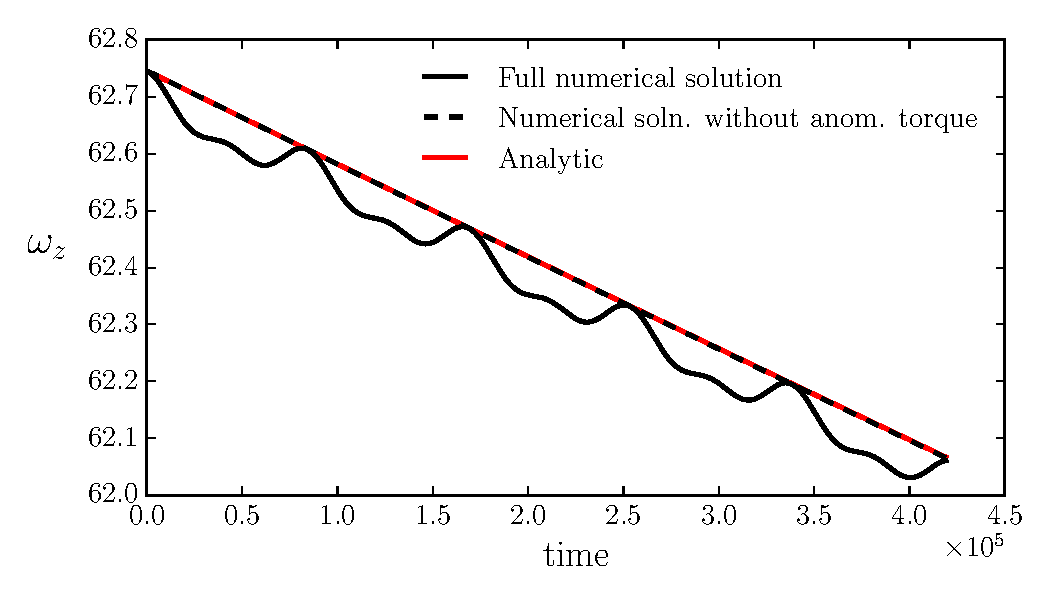
\includegraphics[width=0.7\textwidth]{omegaz.pdf}
%\caption{Comparison of three results for the $z$ component of the spin-vector in
%         the body frame. In solid black is shown the full numerical solution, the
%         dashed black line indicates the numerical solution when the anomalous
%         torque component is neglected, in red is shown the analytic result of
%         equation \eqref{eqn: wz with torque}}
%\label{fig: wz with torque}
%\end{figure}

This result holds for any spin-down strength provided the assumptions listed
above are met. However, we can further simplify by working in the weak 
spin-down limit for which $\epsA \ll 1$. Expanding we have
\begin{equation}
\wz(t) \approx \wz(0) - \frac{2R}{3c}\epsA \wz(0)^{3} t + \mathcal{O}(\epsA^{2})
\end{equation}

Now we refer to \citet{Landau1969} where, provided suitable initial conditions
are used, the $\psi$ euler angle is shown to satisfy:
\begin{equation}
\dot{\psi} = -\epsI \wz.
\end{equation}
Plugging in the expanded version of $\wz$ and solving we have
\begin{equation}
\psi(t) = -\epsI\wz(0) t + \frac{R}{3c} \epsA \epsI \omega_{z}(0)^{3} t^{2} + \pi/2 + \mathcal{O}(\epsA^{2})
\end{equation}
%We can also write this in terms of the precession and spin-down time scales:
%\begin{equation}
%\psi(t) = - \frac{t}{\tauP} + \frac{1}{2}\frac{t^{2}}{\tauP \tauS} + \pi/2 + \mathcal{O}(\epsA^{2})
%\end{equation}

\begin{figure}[htb]
\centering
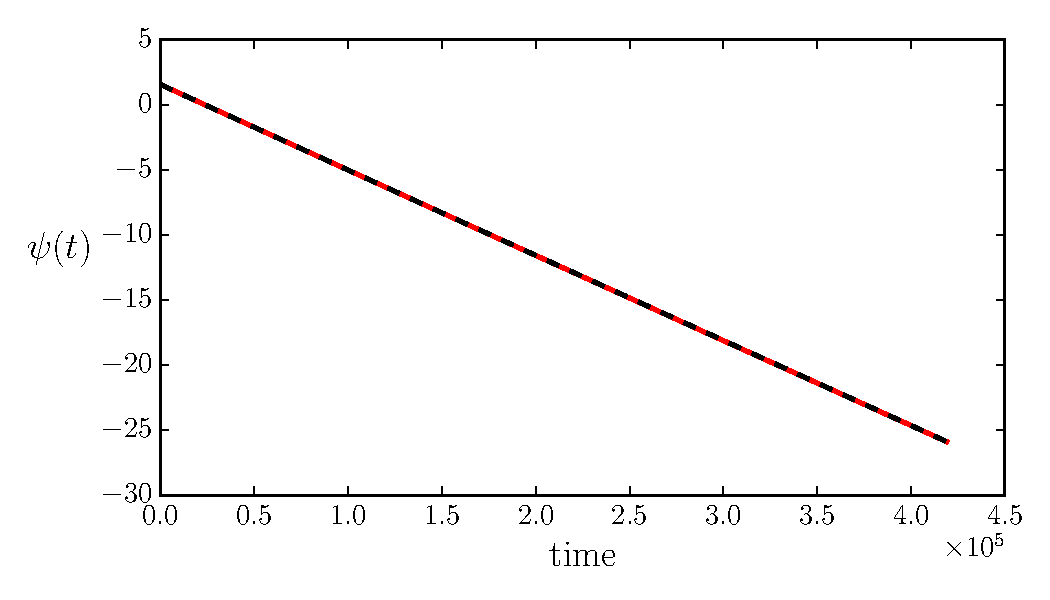
\includegraphics[width=0.7\textwidth]{psi.pdf}
\caption{}
\label{}
\end{figure}

Finally from \citet{Landau1969} again we have
\begin{align}
\dot{\phi} & = \wz - \dot{\psi} = \wz(1 + \epsI). + \mathcal{O}(\theta^{2})
\end{align}
Substituting for $\wz$ and differentiating we have
\begin{align}
\ddot{\phi} = -(1+\epsI)\left(\frac{2R}{3c} \epsA \wz(0)^{3}\right) + \mathcal{O}(\epsA^{2})
\end{align}
%Or
%\begin{align}
%\ddot{\phi} = -(1+\epsI) \frac{wz(0)}{\tauS} + \mathcal{O}(\epsA^{2}) =
%-\frac{\wz(0)}{\tauP} - \frac{1}{\tauP\tauS} + \mathcal{O}(\epsA^{2})
%\end{align}

\subsubsection{Plugging terms into the spin-down}
From \citet{Jones2001}, the instantaneous EM frequency is given by 
\begin{equation}
\Phidot = \dot{\phi} + \dot{\psi} \sin\chi
\frac{\cos\theta\sin\chi - \sin\psi\sin\theta\cos\chi}{
    (\sin\theta\cos\chi - \cos\theta\sin\psi\sin\chi)^{2} + \cos^{2}\psi\sin^{2}\chi}.
\end{equation}
To simplify the calcualtion, we define a function as such
\begin{equation}
f(\theta, \chi, \psi) = \sin\chi
\frac{\cos\theta\sin\chi - \sin\psi\sin\theta\cos\chi}{
    (\sin\theta\cos\chi - \cos\theta\sin\psi\sin\chi)^{2} + \cos^{2}\psi\sin^{2}\chi}.
\end{equation}
Then differentiating the frequency, we get the spin-down:
\begin{align}
\Phiddot = \ddot{\phi} + \ddot{\psi}f(\theta, \chi, \psi) + \dot{\psi}\frac{d}{dt}f(\theta, \chi, \psi)
\end{align}
Since the only time dependence in $f$ is that of $\psi$, we may simplify
\begin{align}
\Phiddot = \ddot{\phi} + \ddot{\psi}f(\theta, \chi, \psi) + \dot{\psi}^{2}\frac{d}{d\psi}f(\theta, \chi, \psi).
\end{align}
Since we know  that $\epsI \ll 1$, we can neglect terms of order $\epsI\epsA$. 
The coefficients then are 
\begin{align}
\ddot{\psi} & = \frac{2R}{3c}\epsA\epsI \wz(0)^{3} + \mathcal{O}(\epsA^{2}) \\
\dot{\psi}^{2} & = \left(\epsI \wz(0)\right)^{2} + \frac{4R}{3c} \epsA \epsI^{2} \wz(0)^{4} t +  \mathcal{O}(\epsA^{2}) \\
\ddot{\phi} & = -(1+\epsI)\left(\frac{2R}{3c} \epsA \wz(0)^{3}\right) + \mathcal{O}(\epsA^{2})
\end{align}

%When $\Tsd=0$, the general solution to Eulers rigid body equations are
%\begin{align}
%\wx &= C_2 \cos(\epsI C_1 t) - C_3 \sin(\epsI C_1 t) \\
%\wy &= C_3 \cos(\epsI C_1 t) + C_2 \sin(\epsI C_1 t) \\
%\wz &= C_1 
%\end{align}
%
%We fix the integration constants by specifying the initial coniditions: as in
%the simulation results we begin with the spin vector $\spin$ in the $x-z$ plane
%at an angle $a_{0}$ to the $z$ axis such that $\wz(0) = \omega_{0}\cos(a_{0})$.
%Under the assumptions made above then we obtain a set of solutions for the
%spin-vector in the body frame:
%\begin{align}
%\wx &= \omega_0 \sin(a_0) \cos(\epsI \wz t)  \\
%\wy &= \omega_0 \sin(a_0) \sin(\epsI \wz t) \\
%\wz &= \left(\frac{4R}{3c} \epsA t + \left(\omega_0 \cos(a_0)\right)^{-2}\right)^{-1/2}
%\end{align}

%\subsection{Euler angles}
%Having obtained approximate solutions for the components of the spin-vector in
%the body frame we now need to use these to find approximate solutions for the
%Euler angles $\theta, \phi, \psi$. This can be done by solving the differential
%equations with these approximate solutions
%\begin{align}
%    \dot{\psi} &= -\wz \epsI \\
%    &= -\epsI\left(\frac{4R}{3c} \epsA t + \left(\omega_0 \cos(a_0)\right)^{-2}\right)^{-1/2}
%\end{align}
%Integrating and using the initial condition $\psi(t=0) = \pi/2$ we get
%\begin{align}
%\psi(t) = \frac{-3\epsI c}{2 R \epsA} 
%          \left(\frac{4R}{3c} \epsA t + \left(\omega_0 \cos(a_0)\right)^{-2}\right)^{1/2}
%          + \frac{\pi}{2} + \frac{3 \epsI c}{2 R \epsA \omega_0 \cos(a_0)}
%\end{align}
%Writing this in terms of $\wz$ we have
%\begin{align}
%\psi(t) = \frac{-3\epsI c}{2 R \epsA} 
%          \left(\frac{1}{\wz} - \frac{1}{\wz(t=0)}\right)
%          + \frac{\pi}{2} 
%\end{align}

\biblio
\end{document}

